%\documentclass[12pt,preprint]{aastex}
%\documentclass[twocolumn]{emulateapj}
%\documentclass[manuscript]{aastex}

\documentclass[useAMS,usenatbib,a4]{mn2e}
%\documentclass[useAMS,usenatbib,a4,referee]{mn2e}
%\documentclass[usenatbib,letterpaper]{mn2e}


% molass11.tex
%\documentclass[nameyear]{elsart}
%\documentclass{elsart}
\usepackage{times}
\usepackage{graphicx,bm,amssymb}
\usepackage{ulem}
\usepackage{epsfig}
\usepackage{amssymb}
\usepackage{natbib}
%\journal{New Astronomy}
\usepackage{psfrag}
\voffset= -0.45in
\setlength{\textheight}{9.5in}
%---------------------------------------------------------------------
% Bibliography and bibfile
\def\aj{AJ}%% Astronomical Journal
\def\actaa{Acta Astron.}%% Acta Astronomica
\def\araa{ARA\&A}%% Annual Review of Astron and Astrophys
\def\apj{ApJ}%% Astrophysical Journal
\def\apjl{ApJ}%% Astrophysical Journal, Letters
\def\apjs{ApJS}%% Astrophysical Journal, Supplement
\def\ao{Appl.~Opt.}%% Applied Optics
\def\apss{Ap\&SS}%% Astrophysics and Space Science
\def\aap{A\&A}%% Astronomy and Astrophysics
\def\aapr{A\&A~Rev.}%% Astronomy and Astrophysics Reviews
\def\aaps{A\&AS}%% Astronomy and Astrophysics, Supplement
\def\azh{AZh}%% Astronomicheskii Zhurnal
\def\baas{BAAS}%% Bulletin of the AAS
\def\bac{Bull. astr. Inst. Czechosl.}%% Bulletin of the Astronomical Institutes of Czechoslovakia
\def\caa{Chinese Astron. Astrophys.}%% Chinese Astronomy and Astrophysics
\def\cjaa{Chinese J. Astron. Astrophys.}%% Chinese Journal of Astronomy and Astrophysics
\def\icarus{Icarus}%% Icarus
\def\jcap{J. Cosmology Astropart. Phys.}%% Journal of Cosmology and Astroparticle Physics
\def\jrasc{JRASC}%% Journal of the RAS of Canada
\def\mnras{MNRAS}%% Monthly Notices of the RAS
\def\memras{MmRAS}%% Memoirs of the RAS
\def\na{New A}%% New Astronomy
\def\nar{New A Rev.}%% New Astronomy Review
\def\pasa{PASA}%% Publications of the Astron. Soc. of Australia
\def\pra{Phys.~Rev.~A}%% Physical Review A: General Physics
\def\prb{Phys.~Rev.~B}%% Physical Review B: Solid State
\def\prc{Phys.~Rev.~C}%% Physical Review C
\def\prd{Phys.~Rev.~D}%% Physical Review D
\def\pre{Phys.~Rev.~E}%% Physical Review E
\def\prl{Phys.~Rev.~Lett.}%% Physical Review Letters
\def\pasp{PASP}%% Publications of the ASP
\def\pasj{PASJ}%% Publications of the ASJ
\def\qjras{QJRAS}%% Quarterly Journal of the RAS
\def\rmxaa{Rev. Mexicana Astron. Astrofis.}%% Revista Mexicana de Astronomia y Astrofisica
\def\skytel{S\&T}%% Sky and Telescope
\def\solphys{Sol.~Phys.}%% Solar Physics
\def\sovast{Soviet~Ast.}%% Soviet Astronomy
\def\ssr{Space~Sci.~Rev.}%% Space Science Reviews
\def\zap{ZAp}%% Zeitschrift fuer Astrophysik
\def\nat{Nature}%% Nature
\def\iaucirc{IAU~Circ.}%% IAU Circulars
\def\aplett{Astrophys.~Lett.}%% Astrophysics Letters
\def\apspr{Astrophys.~Space~Phys.~Res.}%% Astrophysics Space Physics Research
\def\bain{Bull.~Astron.~Inst.~Netherlands}%% Bulletin Astronomical Institute of the Netherlands
\def\fcp{Fund.~Cosmic~Phys.}%% Fundamental Cosmic Physics
\def\gca{Geochim.~Cosmochim.~Acta}%% Geochimica Cosmochimica Acta
\def\grl{Geophys.~Res.~Lett.}%% Geophysics Research Letters
\def\jcp{J.~Chem.~Phys.}%% Journal of Chemical Physics
\def\jgr{J.~Geophys.~Res.}%% Journal of Geophysics Research
\def\jqsrt{J.~Quant.~Spec.~Radiat.~Transf.}%% Journal of Quantitiative Spectroscopy and Radiative Trasfer
\def\memsai{Mem.~Soc.~Astron.~Italiana}%% Mem. Societa Astronomica Italiana
\def\nphysa{Nucl.~Phys.~A}%% Nuclear Physics A
\def\physrep{Phys.~Rep.}%% Physics Reports
\def\physscr{Phys.~Scr}%% Physica Scripta
\def\planss{Planet.~Space~Sci.}%% Planetary Space Science
\def\procspie{Proc.~SPIE}%% Proceedings of the SPIE
\let\astap=\aap
\let\apjlett=\apjl
\let\apjsupp=\apjs
\let\applopt=\ao
%


%---------------------------------------------------------------------


\newcommand{\zsun}{\mbox{$Z_\odot$}}
\newcommand{\msun}{\mbox{$M_\odot$}}
\newcommand{\rsun}{\mbox{$R_\odot$}}
\def\be{\begin{equation}}
\def\ee{\end{equation}}
\def\bary{\begin{eqnarray}}
\def\eary{\end{eqnarray}}

\def\bi{\begin{itemize}}
\def\ei{\end{itemize}}
\def\lsim{\mathrel{\rlap{\lower3pt\hbox{\hskip1pt$\sim$}}
     \raise1pt\hbox{$<$}}} %less than or approx. symbol
\def\gsim{\mathrel{\rlap{\lower3pt\hbox{\hskip1pt$\sim$}}
     \raise1pt\hbox{$>$}}} %greater than or approx. symbol
\def\la{\langle}
\def\ra{\rangle}

\def\cal{\it}

%\def\COrate{$^{12}$C($\alpha,\gamma$)$^{16}$O\ }
%\newcommand{\ud}[2]{\mbox{$^{+ #1}_{- #2}$}}


%---------------------------------------------------------------------

\begin{document}
\title[Emission processes and  Ultra High Energy Cosmic Rays  from NGC1275?]
{Emission processes and  Ultra High Energy Cosmic Rays  from NGC1275?}
% Force line breaks with \\
%\author[N. Fraija et al.]
%%
%{Nissim Fraija$^1$ \thanks{E-mail:nifraija@astro.unam.mx. Luc Binette-Fundaci\'on UNAM Fellow.}\\
  %Uriel Luviano $^2$
%$^1$Instituto de Astronom\' ia, Universidad Nacional Aut\'onoma de M\'exico, Circuito Exterior,
%\\C.U., A. Postal 70-264, 04510 M\'exico D.F., M\'exico
%
%$^2$Facultad de Ciencias, Universidad Nacional Aut\'onoma de M\'exico, Circuito Exterior,
%\\C.U., A. Postal 70-264, 04510 M\'exico D.F., M\'exico
%
%}\\

\author[N. Fraija et al.]
  {N.~Fraija,$^1$\thanks{E-mail:nifraija@astro.unam.mx. Luc Binette-Fundaci\'on UNAM Fellow.}
    U.~Luviano,$^2$\\
    $^1$Instituto de Astronom\' ia, Universidad Nacional Aut\'onoma de M\'exico, Circuito Exterior,
C.U., A. Postal 70-264, 04510 M\'exico D.F., M\'exico\\
        $^2$Facultad de Ciencias, Universidad Nacional Aut\'onoma de M\'exico, Circuito Exterior,
C.U., A. Postal 70-264, 04510 M\'exico D.F., M\'exico}

%\author[N. Fraija et al.]
  %{Nissim Fraija,$^1$\thanks{E-mail:nifraija@astro.unam.mx. Luc Binette-Fundaci\'on UNAM Fellow.}
    %Uriel Luviano,$^2$\\
%
%$^1$Instituto de Astronom\' ia, Universidad Nacional Aut\'onoma de M\'exico, Circuito Exterior,
%C.U., A. Postal 70-264, 04510 M\'exico D.F., M\'exico\\
%$^2$Facultad de Ciencias, Universidad Nacional Aut\'onoma de M\'exico, Circuito Exterior,
%C.U., A. Postal 70-264, 04510 M\'exico D.F., M\'exico}


%\date{\today} % It is always \today, today,
             %  but any date may be explicitly specified

\maketitle
	
\begin{abstract}
%
Long gamma-ray bursts have been widely associated with collapsing massive stars in the framework of   collapsar model.    High-energy neutrinos and photons can be produced in the internal shocks of middle relativistic jets from core-collapse supernova.  Although photons can hardly escape, high-energy neutrinos could be the only signature when the jets are hidden.  We show that using suitable parameters, high-energy neutrinos in GeV - PeV range  can be produced in the hidden jet inside the collapsar, thus demonstrating that these objects are candidates to produce neutrinos with energies between  1 - 10 PeV  which were observed with IceCube.  On the other hand, due to matter effects, high-energy neutrinos may oscillate resonantly from one flavor to another before leaving the star. Using two (solar, atmospheric and accelerator parameters) and three neutrino mixing, we study the possibility of resonant oscillation for these neutrinos created in internal shocks. Also we compute the probabilities of neutrino oscillations in the matter at different distances along the jet (before leaving the star) and after in vacuum, on their path to Earth.   Finally, neutrino flavor ratios on Earth are estimated. 
  
%PACS numbers may be entered using the \verb+\pacs{#1}+ command.
\end{abstract}
\begin{keywords}
Long Gamma-ray burst: High-energy Neutrinos:  -- Neutrino Oscillation
\end{keywords}


%\pacs{98.70.Rz; 98.70.Sa}% PACS, the Physics and Astronomy
                       % Classification Scheme.
%\keywords{Suggested keywords}%Use showkeys class option if keyword
                              %display desired
%\maketitle


\section{Introduction}



NGC 1275, also known as Perseus A and 3C 84, is the nearby active galaxy located at the centre of the Perseus cluster at  redshift of $z=0.0179$.   This source has a strong, compact nucleus which has been studied in detail with very long baseline interferometry (VLBI)\cite{ver94, tay06, wal00, asa06}.  These observations reveal a compact core and a bowshock-like souther jet component moving steadily outwards  
at 0.3 mas/year \cite{kel04,lis09}.  The norther counter jet is also detected, though it is much less prominent due to Doppler dimming, as well as to free-free absorption due an intervening disk.    Walker, Romney and Berson (1994) derive from these observations that the jet has an intrinsic velocity of $0.3c - 0.5c$ oriented at an angle $\approx$ 30$^\circ$ - 55$^\circ$ to the line of sight.  Polarization has recently been detected in the southern jet\cite{tay06}, suggesting increasingly strong interactions of the jet with the surrounding environment\cite{abd09a}.\\   
Perseus furthermore hosts a luminous radio mini halo - a diffuse synchrotron emission that fills a large fraction of the cluster core region - and shows a source extension of $\approx$200 kpc \cite{ped90}.  This radio mini-halo is well modeled by the hadronic scenario where the radio emitting electrons are produced in hadronic CR proton interaction with ambient gas protons requiring only a very modest fraction of  few percent CR pressure relative to thermal pressure \cite{pfr04}.   These conditions provide high target densities for hadronic CRp-p interactions and enhance the resulting $\gamma$-ray flux \cite{ale10}. This source has been detected by MAGIC telescopes with a statistical significance of $6.6\,\sigma$ above 100 GeV in 46 hr of stereo observations carried out between August 2010 and February 2011.  The measured differential energy spectrum between 70 GeV and 500 GeV can be described by a power law with a steep spectral index of $\Gamma=-4.1\pm0.7_{stat}\pm0.3_{syst}$, and the average flux above 100 GeV is $F_{\gamma}=1.3\pm 0.2_{stat}\pm0.3_{syst}\times 10^{-11}\,cm^{-2}\,s^{-1}$ \cite{ale12}.  





It has been proposed that astrophysical sources accelerating ultra high energy cosmic rays (UHECRs) also could produce
high energy $\gamma$-rays by proton interactions with photons at the source and/or the surrounding radiation and matter.  Hence, VHE photons detected from Cen A could be the result of hadronic interactions of cosmic rays accelerated by the jet with photons radiated inside the jet 
or protons in the lobes \citep{gop10, rie09, kac09a, kac09b, rom96, iso02, hon09, abd10, der09}.

Pierre Auger Observatory (PAO) studied the spectra of UHECR above $57$ EeV through their shower properties finding a mixed composition of $p$ and $Fe$ \citep{yam07, abr08, ung07}.  By contrast,  HiRes data are consistent with a dominant proton composition at those energies, but uncertainties in the shower properties  \citep{ung07} and in the particle physics extrapolated to this extreme energy scale \citep{eng07} preclude definitive statements about the composition. At least two events of the UHECRs observed by PAO were detected \citep{abr07,abr08} inside of a $3.1^{\circ}$ circle centered at Cen A.



Synchrotron/Synchrotron-Self Compton (SSC) models have been very successful in explaining the multiwavelength emission from Broad-Line Lacertae (BL Lac) objects \citep{blo96, tav98}. If FRIs are misaligned BL Lac objects, then one would  expect synchrotron/SSC to explain their non-thermal spectral energy distribution (SED) as well. In the synchrotron/SSC scenario the low energy  emission, radio through optical, originates from synchrotron radiation while high energy emission, X-rays through VHE $\gamma$-rays, originates from SSC.  
However, many blazars have higher energy synchrotron peaks,  so this mechanism then covers much of the X-ray band; for them only the $\gamma$-rays come from SSC mechanism. In Cen A, synchrotron/SSC model has been applied successfully to fit the two main peaks of the SED, jointly or separated, with one or more electron populations \citep{abd10, chi01, len08, ore09, har09}.   On the other hand, some authors \citep{der09, gup08, bec09} have considered  hadronic processes to explain the VHE photons apparent in the SED. 


In this work we use the fact  that leptonic processes are insufficient to explain the entire spectrum of NGC1275, and introduce hadronic processes that may
leave a signature in the number of UHECRs observed on Earth.  Our contribution is to describe jointly the SED of NGC1275 as well as the observed number of UHECR by PAO. We first require a description of the SED up to the highest energies obtaining parameters as:  proton spectral index ($\alpha_p$),  proton proportionality constant ($A_p$) and  the normalization energy ($E_0$). Then, we use these parameters to estimate the expected UHECRs observed by PAO. The main assumption here, is the continuation of the proton spectrum to ultra high energies. We also estimate the neutrino expectation in a hypothetical Km$^3$ telescope when considering that the VHE photons in the SED of Cen A  are produced by pp interaction. 

%The organization of the paper is as follows: In section 2, we give  a briefly summarize  about Pierre Auger Observatory and related the geometry quantities of the detector with the observables of a protron power  law,  in section 3, we follow a Leptonic model (synchrotron/SSC) to  describe  both peaks, we calculate the magnetic field, the electrons Lorentz factors and   the synchrotron/SSC photon energies. The hadronic  model is showed in section 4, where we consider that  VHE photons were coming from  interactions of accelerating protons  with  photons ($\sim$ 150 keV ) and  from interaction of accelerating protons  with  the thermal proton density in the  lobes. In the section 5, we show all free and fixed parameters  used to fit all electromagnetic spectrum and also the expected UHECRs on earth. In section 6, we extrapolate the possible neutrino spectrum and calculate de signal to noise ratio for an hypothetical  km$^3$ neutrino Telescope In section 7,  briefly discussion and conclusions are given. 


\section{Jet Dynamics}


\section{Leptonic Model}

\subsection{Synchrotron self-Compton}


%
The non-thermal radio emission  can be inferred through synchrotron radiation  generated  by an electron distribution.  The population of  these accelerated electrons  can be described by a broken power-law given by \citep{1994hea2.book.....L,  2001MNRAS.326.1499H, 2006MNRAS.368L..15H, 2011MNRAS.415..133H}
%
\begin{equation}
\label{espele}
N_e(\gamma_e)   = A_e
\cases {
\gamma_e^{-\alpha} 						& 	$\gamma_{e,m}<\gamma_e < \gamma_{e,b}$,\cr
\gamma_{e,b}    \gamma_e^{-(\alpha+1)}          & 	$\gamma_{e,b} \leq  \gamma_e<\gamma_{e,max}$,\cr
}
\end{equation}
%
\noindent where  $A_e$ is the proportionality electron constant, $\alpha$ is the spectral index and $\gamma_{e,i}$ are  the electron Lorentz  factors. The index $i$ is m, b or max for minimum, break and maximum, respectively.  Assuming an equipartition of energy density  between magnetic field  $U_B=B^2/8\pi$ and electrons $U_e=m_e \int\gamma_e N_e(\gamma_e)d\gamma_e$, the electron Lorentz factors are
%
\bary\label{lorentz}
\gamma_{e,m}&=&\frac{(\alpha-2)}{m_e(\alpha-1)}\,\frac{U_e}{N_e}\cr
\gamma_{e,b}&=& \frac{3\,m_e}{4\,\sigma_T\beta^2} \,  U_B^{-1}\,t^{-1}_{syn}  \cr
\gamma_{e,max}&=&\biggl(\frac{9\, q_e^2}{8\pi\, \sigma_T^2\,\beta^4}\biggr)^{1/4}\,U_B^{-1/4},
\eary 
%
\noindent  where  the constants  $m_p$, $m_e$, $q_e$ and $\sigma_T$ are the proton and electron mass, the electric charge and  Thomson cross section, respectively,  $\beta=v/c\sim 1$ and $z$=0.00183 is the redshift\citep{1998A&ARv...8..237I}.  The observed photon energies, ${\small \epsilon_\gamma^{obs}(\gamma_e)=\sqrt{\frac{8\pi q_e^2}{m_e^2}} (1+z)^{-1}\,\delta_D\, U_B^{1/2}\, \gamma^2_{e,i}}$,  for each Lorentz factor  (eq. \ref{lorentz}) are
%
\begin{eqnarray}\label{synrad}
\epsilon^{obs}_{\gamma,m} &=& \frac{\sqrt{8\pi}\,q_e(\alpha-2)^2}{m_e^3\,(\alpha-1)^2}\,(1+z)^{-1}\,\delta_D\,U_B^{1/2}\, U_e^2 N_e^{-2},\cr
\epsilon^{obs}_{\gamma,c} &=&\frac{ 9\sqrt{2\pi}\,q_e\,m_e}{8\,\sigma_T^2\beta^4} (1+z)^{-1}\,\delta_D\, U_B^{-3/2}\, t_{syn}^{-2},\cr
\epsilon^{obs}_{\gamma, max} &=&\frac{3\,q_e^2}{m_e\,\sigma_T\,\beta^2} (1+z)^{-1}\, \delta_D,
\end{eqnarray}
%
where we have applied the synchrotron cooling time scale,
\be
t_{syn}=\frac{E'_e}{(dE_e/dt)'}=\frac{3m_e^2}{4\sigma_T\beta^2}U_B^{-1}\,E^{'-1}_e
\ee
% 
and $\delta_D$ is the Doppler factor.  On the other hand, we have that the synchrotron spectrum is obtained  by the shape of the electron spectrum (eq. \ref{espele}) rather than  the emission spectrum of a single particle. Therefore, the energy radiated in the range $\epsilon_\gamma$ to $\epsilon_\gamma + d\epsilon_\gamma$ is given by electrons between   $E_e$ and $E_e + dE_e$, then we can estimate the photon spectrum through emissivity $\epsilon_\gamma N_\gamma(\epsilon_\gamma) d\epsilon_\gamma=\biggl(- \frac{dE_e}{dt}\biggr)\,N_e(E_e)dE_e$.  Following  \cite{1994hea2.book.....L} and \cite{1986rpa..book.....R}, it is easy to show that if electron distribution has  spectral indexes  $\alpha$ and $(\alpha-1)$, then the photon distribution has  spectral indexes $p=(\alpha-1)/2$ and $p=\alpha/2$, respectively. The proportionality constant is estimated  calculating the total number of radiating electrons  in the actual volume, ${\small n_e=N_e/V=4\pi N_e\,r_d^3/3}$, the maximum radiation power   ${\small P^{obs}_{\nu,max}\simeq  \frac{dE/dt}{\epsilon_\gamma(\gamma_e)}}$ and the distance D$_z$ from the source. Then,  we can obtain the observed synchrotron spectrum as follow
%

\begin{equation}
\label{espsyn}
  \epsilon^2_\gamma N_{\gamma,syn}(\epsilon_{\gamma}) = A_{syn,\gamma}
\cases {
(\frac{\epsilon_\gamma}{\epsilon_{\gamma,m,syn}})^{4/3}                                                                                                  \cr  
 (\frac{\epsilon_\gamma}{\epsilon_{\gamma,m,syn}})^{-(\alpha-3)/2}                                                                                       \cr  
(\frac{\epsilon_{\gamma,c,syn}}{\epsilon_{\gamma,m,syn}})^{-(\alpha-3)/2}    (\frac{\epsilon_\gamma}{\epsilon_{\gamma,c,syn}})^{-(\alpha-2)/2},          \cr  
}\\

$\epsilon^{obs}_\gamma < \epsilon^{obs}_{\gamma,m,syn}$,\\
$\epsilon^{obs}_{\gamma,m,syn} < \epsilon^{obs}_\gamma < \epsilon^{obs}_{\gamma,c,syn}$,\\
$\epsilon^{obs}_{\gamma,c,syn} < \epsilon^{obs}_\gamma < \epsilon^{obs}_{\gamma,max,syn} $\\

\end{equation}
%
\noindent where
\be
\label{Asyn}
 A_{syn,\gamma}= \frac{P^{obs}_{\nu,max} n_e}{4\pi D_z^2}\,\epsilon^{obs}_{\gamma,m} \simeq \frac{8\pi\sigma_T\,\beta^2\,(\alpha-2)^2}{9\,m^2_e\,(\alpha-1)^2\,D_z^2}(1+z)^{-2}\,\delta^2_D\,U_B\,U^2_e\,N_e\,r_d^3
\ee
%
%
It is important to clarify that $r_d$ is the region where emitting electrons  are confined.  \noindent Eq. \ref{espsyn} represents the peak at lower energies (radio wavelength) of the  SED for each of the lobes. 


\begin{equation}
\label{espsyn}
\epsilon^2_{\gamma}
 N_{\gamma,ssc}(\epsilon_\gamma) = A_{ssc,\gamma}
\cases {
(\frac{\epsilon_\gamma}{\epsilon_{\gamma,m,ssc}})^{4/3}    &  $\epsilon^{obs}_\gamma < \epsilon^{obs}_{\gamma,m,ssc}$,\cr
 (\frac{\epsilon_\gamma}{\epsilon_{\gamma,m,ssc}})^{-(\alpha-3)/2}  &  $\epsilon^{obs}_{\gamma,m,ssc} < \epsilon^{obs}_\gamma < \epsilon^{obs}_{\gamma,c}$,\cr
(\frac{\epsilon_{\gamma,c,ssc}}{\epsilon_{\gamma,m,ssc}})^{-(\alpha-3)/2}    (\frac{\epsilon_\gamma}{\epsilon_{\gamma,c,ssc}})^{-(\alpha-2)/2},           &  $\epsilon^{obs}_{\gamma,c,ssc} < \epsilon^{obs}_\gamma < \epsilon^{obs}_{\gamma,max,ssc} $\cr
}
\end{equation}




\section{Hadronic Model}

Some authors \citep{oli00, bha00,sta04,cha09b} have considered possible different mechanisms where protons up to ultra high energies can be accelerated. Thus, we suppose that Cen A is capable of accelerating protons up to ultra high energies with a power law injection spectrum \citep{gup08},

\be\label{spepr}
\frac{dN_p}{dE_p}=A_p\,E_p^{-\alpha_p}
\ee

\noindent where $\alpha_p$ is the proton spectral index and $A_p$ is the proportionality constant.   Energetic protons in the jet mainly lose energy   by p$\gamma$  and pp interactions  \citep{ste68, ber90,bec09,ato03,cha09b}; as described  in the following subsections. 
 

\subsection{p$\gamma$ interaction}

 The p$\gamma$; interaction takes place when accelerated protons collide with  target photons.  The single-pion production channels are $p+\gamma\to n+\pi^+$ and $p+\gamma\to p+ \pi^0$, where the relevant pion decay chains are $\pi^0\to 2\gamma$, $\pi^+\to \mu^++\nu_\mu\to e^++\nu_e+\bar{\nu}_\mu+\nu_\mu$ and $\pi^-\to \mu^-+\bar{\nu}_\mu\to e^-+\bar{\nu}_e+\nu_\mu+\bar{\nu}_\mu$ \citep{ato03}.


In this analysis we suppose  that protons interact with SSC photons ($\sim$ 150 keV) in the same knot. If so, the optical depth is given as $\tau_{p,ssc}\approx r_d\,\theta_{jet}\,\Gamma\, n^{obs}_{\gamma ssc} \sigma_{p\gamma}$, where  $r_d$ is the value of the dissipation radius \citep{bat03}, $\theta_{jet}$ is the jet aperture angle, $\sigma_{p\gamma}=0.9$ mbarn is the cross section  for the production of the delta-resonance in proton-photon interactions and  $n^{obs}_{\gamma ssc}$ is the particle density of SSC photons  into the observer frame \citep{bec09} given by,

\be
n^{obs}_{\gamma ssc}\approx \frac{\epsilon_{knot}\, L^{obs}}{4\pi\,r^2_d\,E^{obs}_{\gamma,c}}
\ee

Assuming that the luminosity of a knot along the jet is a fraction $\epsilon_{knot}\approx 0.1$ of the observed luminosity $L^{obs}=5\times 10^{43}\,erg\,s^{-1}$ for $E^{obs}_{\gamma,c}$ keV, the optical depth is,

\be
\tau_{p,ssc}\approx   \,\Gamma^{-1}\,\biggl(\frac{\theta_{\rm{jet}}}{0.3}\biggr)\,\biggl(\frac{\epsilon_{\rm{knot}}}{0.1}\biggr)\,\biggl( \frac{ L^{obs} } {6 \times10^{43}\,\rm{erg\, s^{-1}} } \biggr)\,\biggl( \frac{ r_d } {10^{16}\,\rm{cm} } \biggr)^{-1}\,\biggl( \frac{ E^{obs}_{\gamma,b}} {\,\rm{keV} } \biggr)^{-1}\,.
\ee


The energy lost rate due to pion production is \citep{ste68, ber90},


\begin{equation}
t'_{p,\gamma}=\frac{1}{2\,\gamma_p}\int^\infty_{\epsilon_0}\,d\epsilon\,\delta_\pi(\epsilon)\xi(\epsilon)\,\epsilon\int^\infty_{\epsilon/2\gamma_p}dx\, x^{-2}\,n(x)
\end{equation}


\indent where $n(x)=dn_\gamma/d\epsilon_\gamma (\epsilon_\gamma=x)$, $\sigma_\pi(\epsilon)$ is the cross section of pion production for a photon with energy $\epsilon$ in the proton rest frame, $\xi(\epsilon)$ is the average fraction of energy transferred to the pion,  and $\epsilon_0=0.15$ is the threshold energy, $\gamma_p=\epsilon_p/m^2_p$.




The rate of energy loss,  $t'_{p,\gamma}$,   $f_{\pi^0,p \gamma}\approx t'_d/t'_{p,\gamma}$  (where $t'_d\sim r_d/\Gamma$ is the expansion time scale),  can  be calculated by following Waxman \& Bahcall 1997 formalism.

\begin{equation}
\label{}
f_{\pi^0, p \gamma}\approx \frac{(1+z)^2\,L^{obs}}{8\,\pi\,\Gamma^2\,\delta^2_D\,dt^{obs}\,E^{obs}_{\gamma,b}}\sigma_{\epsilon_{peak}}\,\xi({\epsilon_{peak}})\,\frac{\Delta\epsilon_{peak} }{\epsilon_{peak}}
\cases{
\frac{E^{obs}_p}{E^{obs}_{p,b}}       &  $E^{obs}_{p} < E^{obs}_{p,b}$ \cr
1                                                             &  $E^{obs}_{p} \geq E^{obs}_{p,b}$\cr
}
\end{equation}


Here, $\sigma_{peak} \approx 5\times\,10^{-28}$ cm$^2$ and $\xi({\epsilon_{peak}})\approx 0.2$ are the values of $\sigma$ and $\xi$ at $E_\gamma \approx \epsilon_{peak}$ and $\Delta\epsilon_{peak}  \approx 0.2$ GeV is the peak width.  

The differential spectrum, $dN_\gamma/dE_\gamma$ of the photon-pions produced by  p$\gamma$ interaction  is related to the fraction of 
energy lost through  the equation: $f_{\pi^0}(E_p)\,E_p\,dN_p/dE_p\,dE_p=E_\gamma\,dN_\gamma/dE_\gamma\,dE_\gamma $.  If we take into account  that $\pi^0$ typically carries $20\%$ of the proton's energy and that each produced photon shares the same energy then, we obtain the observed gamma  spectrum through  the  following relationship,

\begin{equation}
\label{pgamma}
\left(E^2\,\frac{dN}{dE}\right)^{obs}_{\pi^0-p\gamma} = A_{p,\gamma}
\cases{
\left(\frac{E^{obs}_{\gamma}}{E_{0}}\right)^{-1} \left(\frac{E^{obs}_{\gamma,c}}{E_{0}}\right)^{-\alpha_p+3}          &   $E^{obs}_{\gamma} < E^{obs}_{\pi^0-\gamma,c}$\cr
\left(\frac{E^{obs}_{\gamma}}{E_{0}}\right)^{-\alpha_p+2}                                                                                        &   $E^{obs}_{\pi^0-\gamma,c} < E^{obs}_{\gamma}$\cr
}
\end{equation}

\noindent where
\be
A_{p,\gamma}=2.25\times 10^{-13}\frac{\delta_D^{\alpha_p} \,E_0^2\,A_p\,(11s.1)^{2-\alpha_p}  e^{-\tau_{\gamma\gamma}}}{(1+z)^\alpha} \,\biggl(\frac{E^{obs}_{\gamma,c}}{\,\rm{keV}}\biggr)^{-1}\,\biggl( \frac{ L^{obs} } {6 \times10^{43}\,\rm{erg\, s^{-1}} } \biggr)\,\biggl(\frac{dt^{obs}}{3.17 \times10^7 s}\biggr)\,\biggl(\frac{d_z}{76\,\rm{Mpc}}\biggr)^{-2}
\ee

\noindent and
\be
E^{obs}_{\pi^0-\gamma,c}=\,\rm{GeV} \frac{\delta_D^2}{(1+z)^2} \biggl(\frac{E^{obs}_{\gamma,b}}{\,\rm{keV}}\biggr)^{-1}
\ee



The eq.  \ref{pgamma} could represent the VHE photon contribution  to the spectrum. 


\subsection{PP interaction}

Hardcastle et al. 2009 argues that the number density of thermal particles within the giants lobes is $n_p\sim 10^{-4}\,cm^{-3}$. If we assume that  the accelerated protons collide with this thermal particle target then, the energy lost rate due to pion production is given by \citep{ato03},


\begin{equation}
t'_{pp}=(n'_p\,k_{pp}\,\sigma_{pp})^{-1}
\end{equation}


\noindent where $\sigma_{pp}=30$ mbarn is the nuclear interaction cross section, $k_{pp}=0.5$ is the inelasticity coefficient and $n'_p$ is the comoving thermal particle density.  The fraction of energy lost by pp is  $f_{\pi^0,pp}\approx t'_d/t'_{pp}$ then,


\begin{equation}
f_{\pi^0 ,pp}=R\,n'_p\,k_{pp}\,\sigma_{pp}
\end{equation}

\noindent where R is the distance to the lobes from the AGN core.

The differential spectrum, $dN_\gamma/dE_\gamma$ of the photon-pions produced by  pp interaction  is related to the fraction of energy lost through the
equation:  $f_{\pi^0 , pp}(E_p)\,E_p\,(\frac{dN_p}{dE_p})\,dE_p=E_\gamma\,(\frac{dN_\gamma}{dE_\gamma})\,dE_\gamma$. Taking into account that  photon carries 18$\%$ of the proton energy,  we have that the observed pp spectrum is given by \citep{gup08},

\begin{equation}
\label{pp}
\left(E^{2}\, \frac{dN}{dE}\right)^{obs}_{\pi^0 - pp}= A_{pp}\, \left(\frac{E^{obs}_{\gamma}}{E_{0}}\right)^{2-\alpha_p}
\end{equation}
where,

\be
A_{pp}=9.97\times 10^{-21}  \frac{\Gamma^2\,\delta_D^2\,E_0^2\,A_p\,e^{-\tau_{\gamma\gamma}}}  {(1+z)^2}\,R_{\rm{kpc}}\,n'_{p,\rm{cm^{-3}}}\,\biggl(\frac{dt^{obs}}{3.17 \times10^7 s}\biggr)^2\,\biggl(\frac{d_z}{76\,\rm{Mpc}}\biggr)^{-2}
\ee


The eq.  \ref{pp} could represent the VHE photon contribution  to the spectrum. 

%%%%%%%%%%%%%%%%%%%%%%%%%%%%

\section{Summary and conclusions}

We have presented a leptonic and hadronic model to describe the broadband photon spectrum of Cen A.  Our model has eight free parameters   (equipartition magnetic field, equipartition electron energy,  bulk Lorentz factor, spectral  index, ratio of expansion time  and proportionality constants).
The leptonic model describes the spectrum up to a few GeV energies while the hadronic model describes the Cen A spectrum at TeV energies.
Two hadronic interactions have been considered, p$\gamma$ and pp interactions. In the first case, the target is considered as SSC photons with energy of $\sim 150$ keV, while in the second case, the target protons are those in the lobes of Cen A. Only one hadronic interaction is considered at the time but in both cases, the proton spectrum is extrapolated up to ultra high energies to estimate the number of UHECR events expected at Earth. We have required a good description of the photon spectrum to obtain values for the quantities required to estimate the UHECR events. 

When p$\gamma$ interaction is considered, the expected number of UHECR obtained is several orders of magnitude above the observed by PAO. However, when pp interaction is considered, the expected number of UHECR is in very good agreement with PAO observations. 

We have also calculated the neutrino event rate from pp interactions observed by a hypothetical Km$^{3}$ neutrino telescope in the Mediterranean sea. We have calculated the signal to noise ratio considering atmospheric and cosmic neutrino ``backgrounds''. We have obtained that the expected signal event rate is below the required one to disentangle the neutrino emission from Cen A from the "backgrounds".




\section*{Acknowledgements}

We thank the referee  for a critical reading of the paper and valuable suggestions. We also thank B. Zhang, K. Murase, William H. Lee, Fabio de Colle, Enrique Moreno and Antonio Marinelli for useful discussions.   NF gratefully acknowledges a Luc Binette-Fundaci\'on UNAM Posdoctoral Fellowship.
 
 

\bibliographystyle{mn2e}
\bibliography{Bib_NGC1275}








\clearpage
\begin{figure}[h!]
 \centering
  %\begin{narrow}{2cm}{0cm}
  % Requires \usepackage{graphicx}
  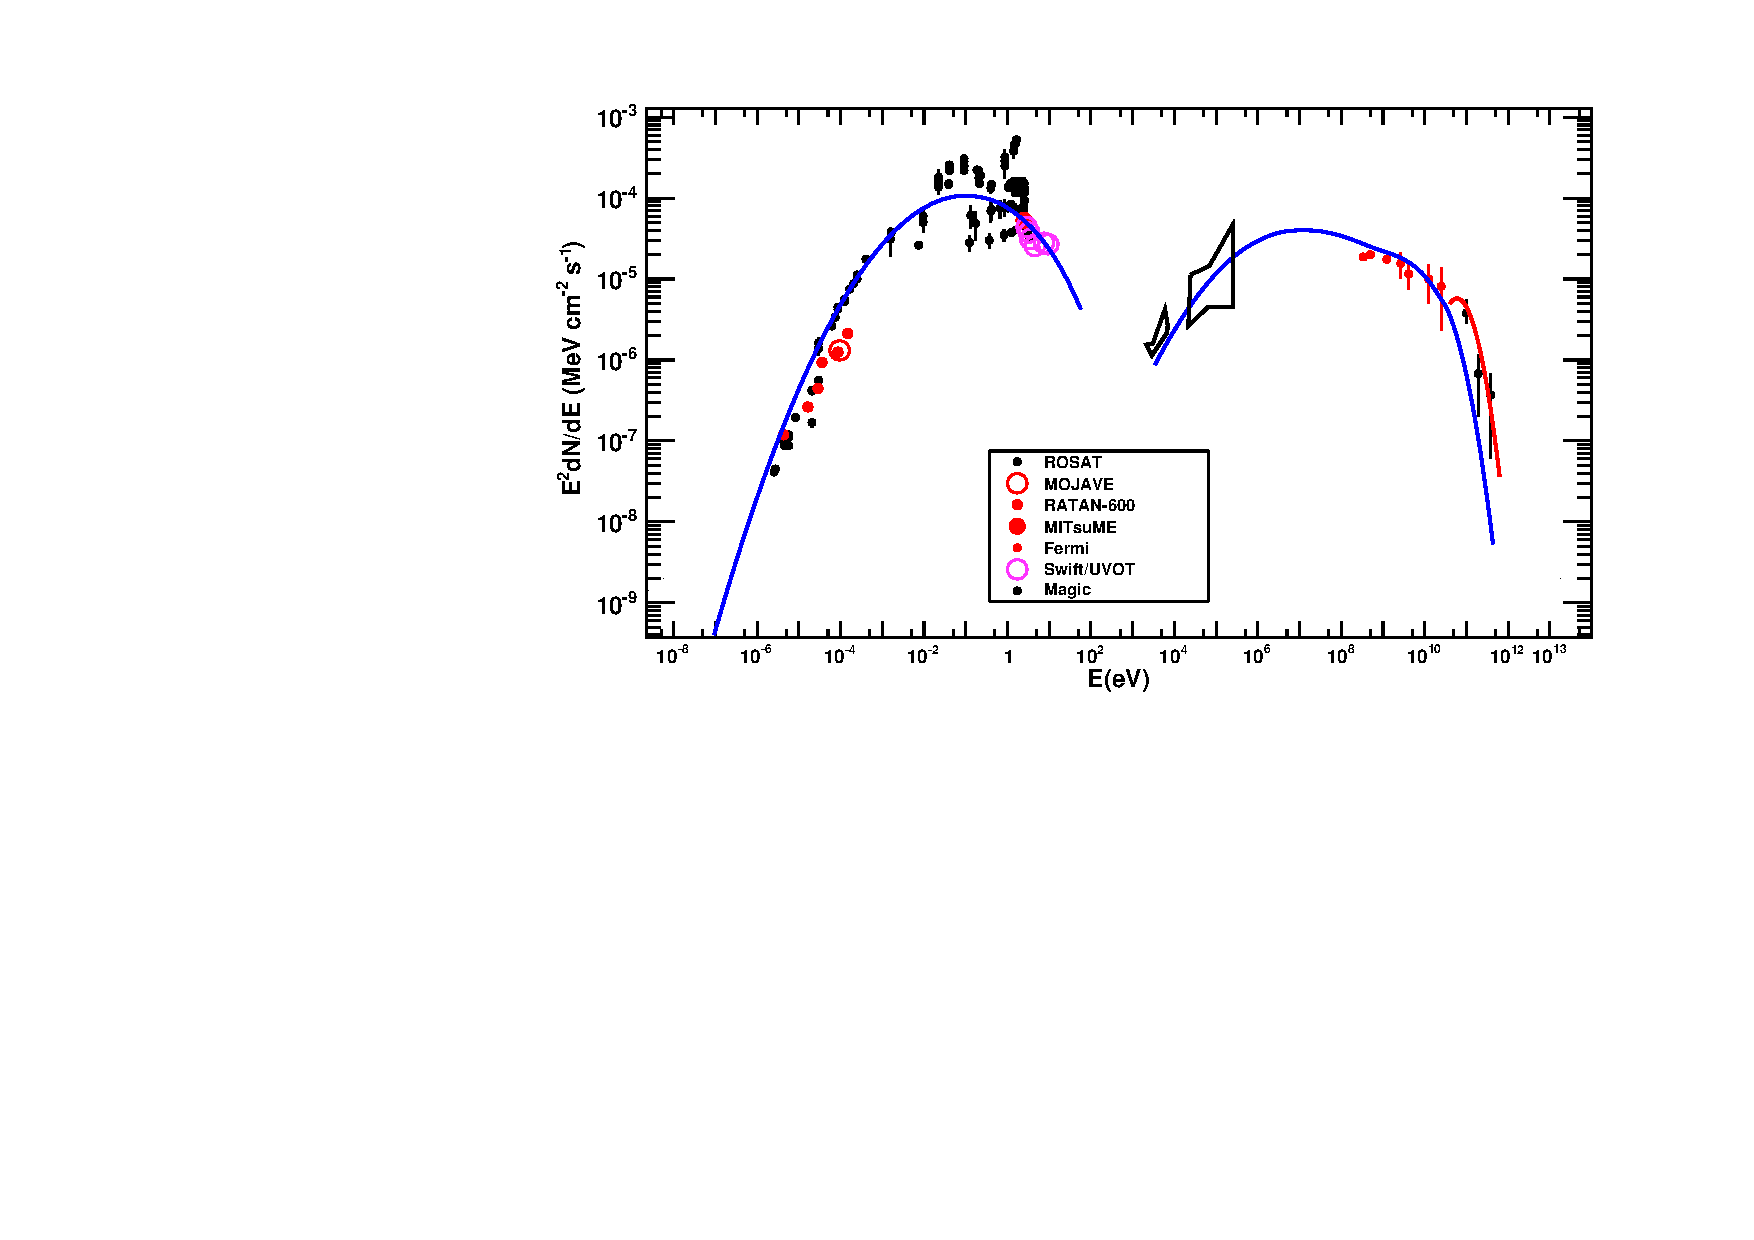
\includegraphics[width=0.7\textwidth]{NGC1275pgamma.pdf}\\
  %\end{narrow}
  \caption{Fitting of observed spectral energy distribution (SED) of NGC1275.  The blue line is a fit to the broadband SED using Fermi data, while the red curve is the p$\gamma$ emission described in section 3.}\label{SEDpgama}
\end{figure} 

\begin{figure}[h!]
 \centering
  %\begin{narrow}{2cm}{0cm}
  % Requires \usepackage{graphicx}
  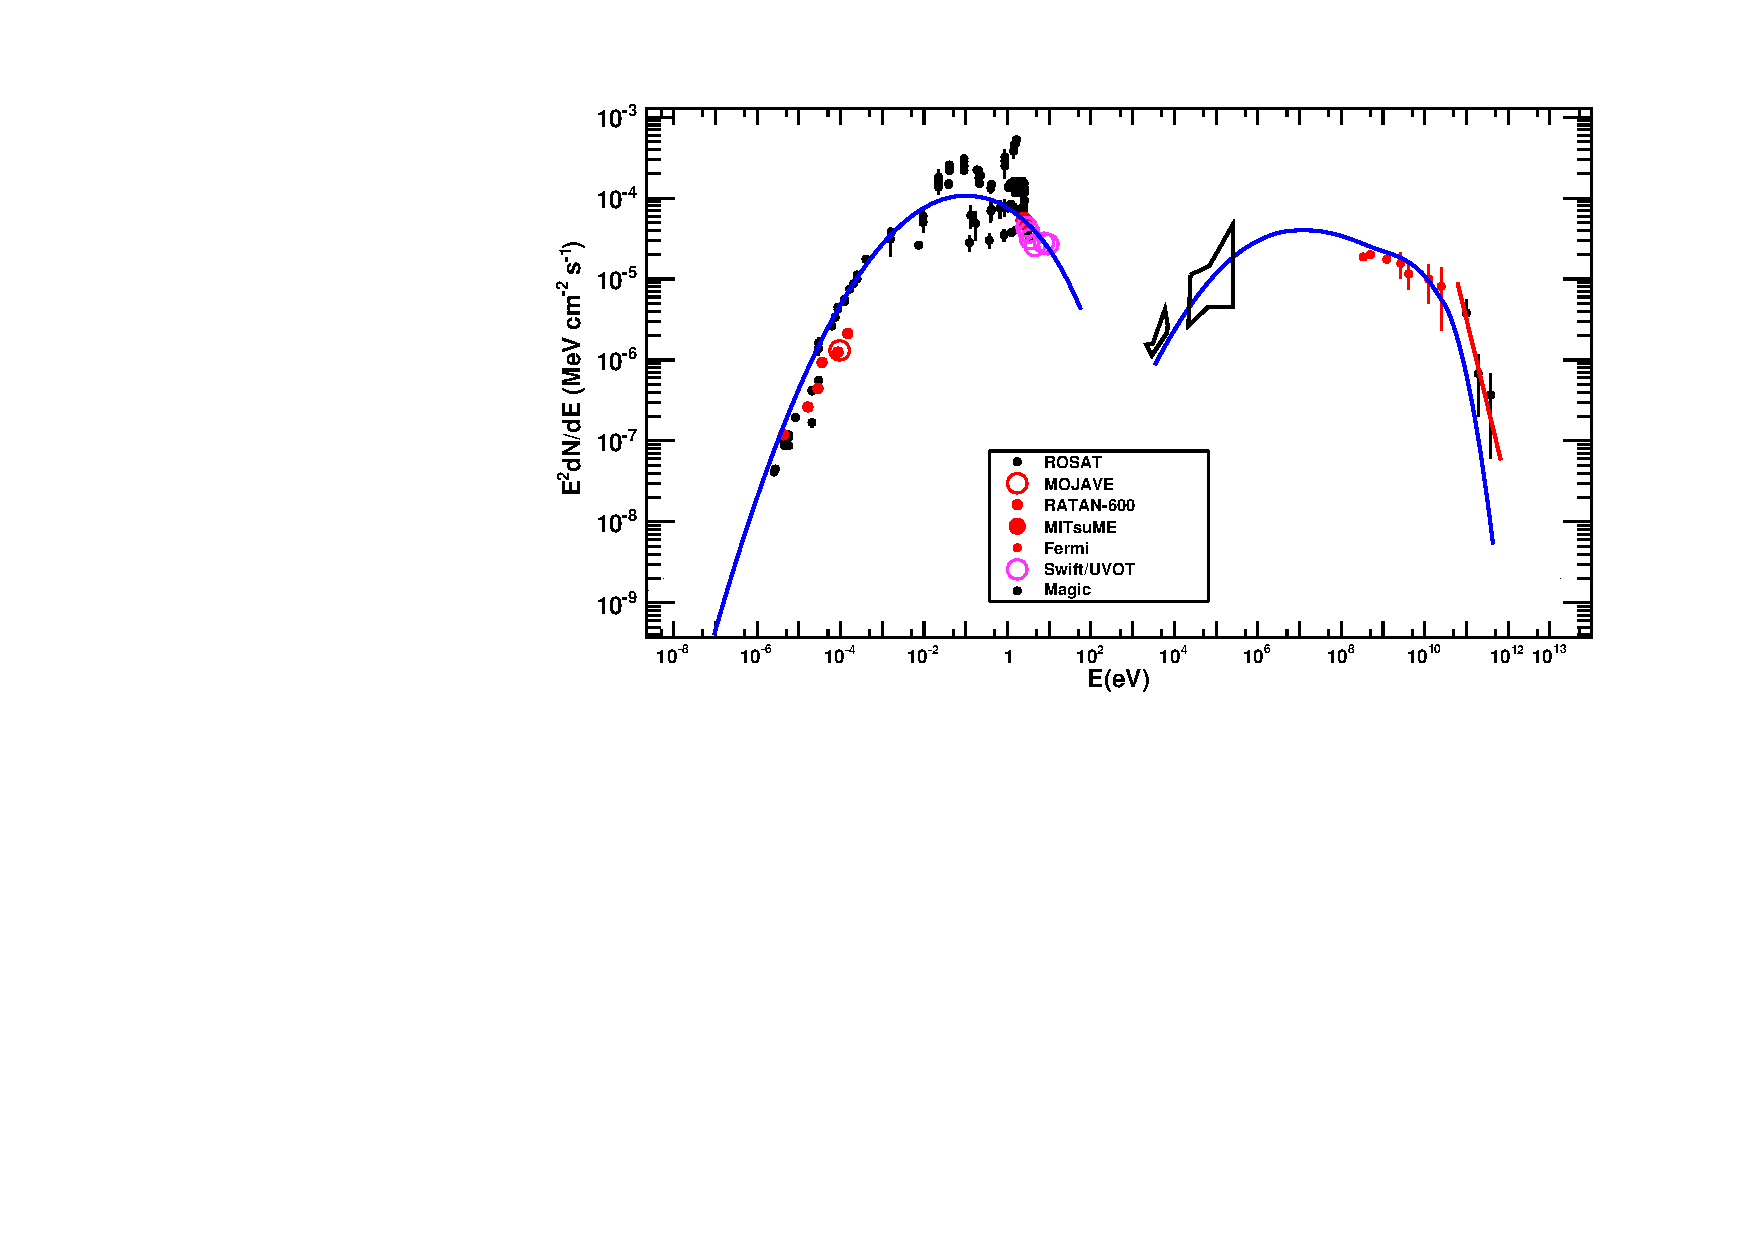
\includegraphics[width=0.7\textwidth]{NGC1275pp.pdf}\\
  %\end{narrow}
  \caption{Fitting of observed spectral energy distribution (SED) of NGC1275.  The blue line is a fit to the broadband SED using Fermi data, while the red curve is the pp emission described in section 3.}\label{SEDpp}
\end{figure} 








\begin{figure}[h!]
 \centering
  %\begin{narrow}{2cm}{0cm}
  % Requires \usepackage{graphicx}
  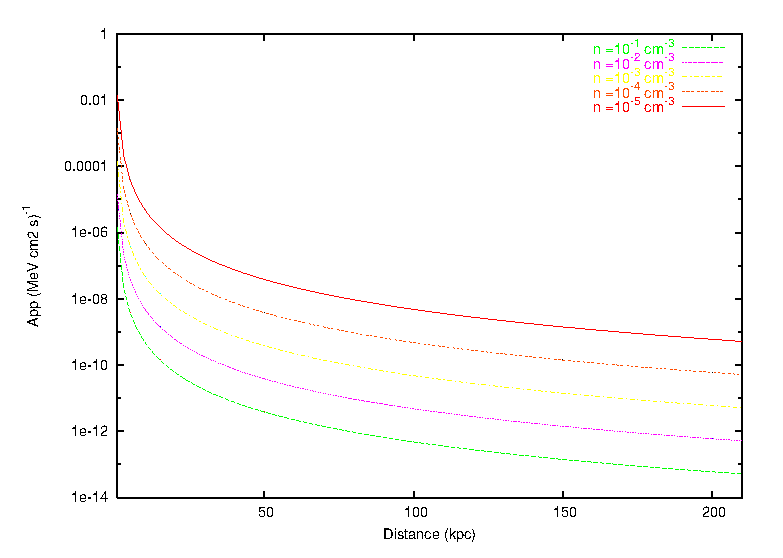
\includegraphics[width=0.7\textwidth]{NGC1275.eps}\\
  %\end{narrow}
  \caption{ App as a function of the Lobes distance for several thermal particle densities for  NGC1275 }\label{densNGC1275}
\end{figure}









%\begin{figure}
 %\epsscale{.80}
%\plotone{cenopticaldepth.eps}
 % \caption{Internal optical depth $\tau_{\gamma\gamma}$ as a function of photon energy $E_\gamma$ for two different luminosities: $L^{obs}=5.0\times 10^{43}$erg/s (solid line) and $L^{obs}=1.0\times 10^{39}$erg/s (dot-dashed line)}
  %\label{optdep}
%\end{figure}


%\begin{figure}
%  \epsscale{.80}
%\plotone{CenAevtRateHESSBartWax.eps}
  % \caption{Neutrino event rate as a function of neutrino energy. The expected Centaurus A event rate for one year of observation with a $Km^{3}$ neutrino telescope assuming the spectrum measured by HESS (black line), the event rate for atmospheric neutrinos (green line) and cosmic neutrinos (purple line) considering the solid angle of $1^{\circ}$ around the sources. A quality cut has been applied to reconstructed events. The integrated number of neutrinos is given for each case.}
   %\label{CenAevtrateHessBartWax}
%\end{figure}




%\begin{figure}
% \epsscale{.80}
%\plotone{visibility.eps}
 % \caption{Calculated the Fraction of Day (FoD) when a source with a given declination is below the horizon with respect to our hypothetical Km$^{3}$ Telescope (solid line) in the Mediterranean and ICECUBE experiments (dashed line). For  Cen A, FoD is $\approx 0.8$ when Km$^{3}$ Telescope is considered. For ICECUBE, Cen A is all the time above the horizon.}
 % \label{fod}
%\end{figure}



\clearpage

\appendix 


\section{Chi-square minimization}
%
Firstly, from pp interaction model  (eq. \ref{pp}),  we fit the $\gamma$-ray spectrum  using two parameters, the proportionality constant of pp spectrum $A_{pp,\gamma}$ (eq. \ref{App}) and the spectral index $\alpha$, as follow.
%
\begin{equation}
\label{ppf}
\left(E^{2}_\gamma\, \frac{dN_\gamma}{dE_\gamma}\right)^{obs}_{\pi^0}=[0]\, \left(\frac{E^{obs}_{\gamma,\pi^0}}{{\rm GeV}}\right)^{2-[1]},
\end{equation}
%
After fitting we obtained the values
%
\begin{center}\renewcommand{\arraystretch}{0.7}\addtolength{\tabcolsep}{-1pt}
\begin{tabular}{ l c c c c}
 \hline \hline
 \scriptsize{} &\scriptsize{Parameter} & \scriptsize{Symbol} & \scriptsize{Value} \\
 \hline
\hline
\scriptsize{Proportionality constant} ($10^{-6}\,{\rm erg/cm^2/s}$)  &\scriptsize{[0]}                    & \scriptsize{$ A_{pp,\gamma} $}  &  \scriptsize{ $3.696\pm 1.014$} \\
\scriptsize{Spectral index}                                                                 &\scriptsize{[1]}                    & \scriptsize{$\alpha$}  & \scriptsize{4.245$\pm$ 0.8838}  \\
\scriptsize{Chi-square/NDF}                                                              & & \scriptsize{$ \chi^2/{\rm NDF}$}  &  \scriptsize{ $0.5335/1.0$} \\

 \hline

\end{tabular}
\end{center}

\begin{center}
\scriptsize{\textbf{Table A1.  The best set of pp interaction parameters for $\gamma$-ray spectrum  of north and south lobes.}}\\
\end{center}
%
Secondly, from synchrotron emission model  (eq.  \ref{espsyn}), we fit  the peak at  radio wavelength using  four parameters,  the proportionality constant of synchrotron $A_{syn,\gamma}$ (eq. \ref{Asyn}), the spectral index $\alpha$, the characteristic and cut-off photon energies $\epsilon^{obs}_{\gamma,m}$   and   $\epsilon^{obs}_{\gamma,c}$ (eq. \ref{synrad}), respectively  as follow 
%
{\small
\begin{equation}
\label{espsynf}
\epsilon^2_\gamma N_\gamma(\epsilon_\gamma) = [0]
\cases {
(\frac{\epsilon_\gamma}{[3]})^{4/3}    &  $\epsilon^{obs}_\gamma < [3]$,\cr
 (\frac{\epsilon_\gamma}{[3]})^{-([1]-3)/2}  &  $[3] < \epsilon^{obs}_\gamma < [2]$,\cr
(\frac{[2]}{[3]})^{-([1]-3)/2}    (\frac{\epsilon_\gamma}{[2]})^{-([1]-2)/2},           &  $[2] < \epsilon^{obs}_\gamma  $\cr
}
\end{equation}
\small}
%
The values of the parameters obtained after fitting
%
\begin{center}\renewcommand{\arraystretch}{0.7}\addtolength{\tabcolsep}{-1pt}
\begin{tabular}{ l c c c c}
  \hline \hline
 \scriptsize{} & \scriptsize{Parameter} &\scriptsize{Symbol} & \scriptsize{Value} \\
 \hline
\hline
\scriptsize{Proportionality constant} ($10^{-5}\,{\rm erg/cm^2/s}$) &\scriptsize{[0]}  & \scriptsize{$ A_{syn,\gamma} $}  &  \scriptsize{ $6.163\pm 0.706$} \\
\scriptsize{Spectral index}                                         &\scriptsize{[1]}                    & \scriptsize{$\alpha$}  &  \scriptsize{ $2.827\pm 0.034$}  \\
\scriptsize{Cut-off photon energy} ($10^{-4}\,{\rm eV}$)                   &\scriptsize{[2]}  & \scriptsize{$ \epsilon^{obs}_{\gamma,c} $}  &  \scriptsize{ $8.507\pm 0.745$} \\
\scriptsize{Characteristic photon energy}  ($10^{-1}\,{\rm eV}$)      &\scriptsize{[3]}   & \scriptsize{$\epsilon^{obs}_{\gamma,m}$}  & \scriptsize{1.00$\pm$ 0.009}  \\
\scriptsize{Chi-square/NDF}                                                             & & \scriptsize{$ \chi^2/{\rm NDF}$}  &  \scriptsize{ $841.2/30$} \\
 \hline
\end{tabular}
\end{center}
\begin{center}
\scriptsize{\textbf{Table A2.  The best set of synchrotron parameters for the peak   at  radio wavelength  of north and south lobes.}}\\
\end{center}


 



%\begin{figure}
%\vspace{0.5cm}
%{ \centering
%\resizebox*{0.45\textwidth}{0.22\textheight}
%{\includegraphics{protonen_time_r1x01.eps}}
%\resizebox*{0.45\textwidth}{0.22\textheight}
%{\includegraphics{protonen_time_r1x001.eps}}
%\resizebox*{0.45\textwidth}{0.22\textheight}
%{\includegraphics{protonen_time_r1x0001.eps}}
%\resizebox*{0.45\textwidth}{0.22\textheight}
%{\includegraphics{protonen_time_r1x00001.eps}}
%}
%\caption{Proton cooling time scales in the comoving frame for different processes as a function of proton energy (E$_p$) when the shell collisions take place  at r=$6\times 10^9$ cm and  different magnetic fields. Synchrotron radiation (t$'_{sync}$), IC+KN scattering (t$'_{ic+KN}$),  Bethe-Heitler (t$'_{BH}$), shock acceleration time (t$'_{acc}$) }
%\label{ptime_r1}
%\end{figure}



\end{document}
